\PassOptionsToPackage{unicode=true}{hyperref} % options for packages loaded elsewhere
\PassOptionsToPackage{hyphens}{url}
%
\documentclass[]{article}
\usepackage{lmodern}
\usepackage{amssymb,amsmath}
\usepackage{ifxetex,ifluatex}
\usepackage{fixltx2e} % provides \textsubscript
\ifnum 0\ifxetex 1\fi\ifluatex 1\fi=0 % if pdftex
  \usepackage[T1]{fontenc}
  \usepackage[utf8]{inputenc}
  \usepackage{textcomp} % provides euro and other symbols
\else % if luatex or xelatex
  \usepackage{unicode-math}
  \defaultfontfeatures{Ligatures=TeX,Scale=MatchLowercase}
\fi
% use upquote if available, for straight quotes in verbatim environments
\IfFileExists{upquote.sty}{\usepackage{upquote}}{}
% use microtype if available
\IfFileExists{microtype.sty}{%
\usepackage[]{microtype}
\UseMicrotypeSet[protrusion]{basicmath} % disable protrusion for tt fonts
}{}
\IfFileExists{parskip.sty}{%
\usepackage{parskip}
}{% else
\setlength{\parindent}{0pt}
\setlength{\parskip}{6pt plus 2pt minus 1pt}
}
\usepackage{hyperref}
\hypersetup{
            pdftitle={Analisis de Variables predictoras - sin ciclocursada},
            pdfauthor={Sebastian Jaremczuk},
            pdfborder={0 0 0},
            breaklinks=true}
\urlstyle{same}  % don't use monospace font for urls
\usepackage[margin=1in]{geometry}
\usepackage{listings}
\newcommand{\passthrough}[1]{#1}
\usepackage{graphicx,grffile}
\makeatletter
\def\maxwidth{\ifdim\Gin@nat@width>\linewidth\linewidth\else\Gin@nat@width\fi}
\def\maxheight{\ifdim\Gin@nat@height>\textheight\textheight\else\Gin@nat@height\fi}
\makeatother
% Scale images if necessary, so that they will not overflow the page
% margins by default, and it is still possible to overwrite the defaults
% using explicit options in \includegraphics[width, height, ...]{}
\setkeys{Gin}{width=\maxwidth,height=\maxheight,keepaspectratio}
\setlength{\emergencystretch}{3em}  % prevent overfull lines
\providecommand{\tightlist}{%
  \setlength{\itemsep}{0pt}\setlength{\parskip}{0pt}}
\setcounter{secnumdepth}{0}
% Redefines (sub)paragraphs to behave more like sections
\ifx\paragraph\undefined\else
\let\oldparagraph\paragraph
\renewcommand{\paragraph}[1]{\oldparagraph{#1}\mbox{}}
\fi
\ifx\subparagraph\undefined\else
\let\oldsubparagraph\subparagraph
\renewcommand{\subparagraph}[1]{\oldsubparagraph{#1}\mbox{}}
\fi

% set default figure placement to htbp
\makeatletter
\def\fps@figure{htbp}
\makeatother

\usepackage{booktabs}
\usepackage{longtable}
\usepackage{array}
\usepackage{multirow}
\usepackage{wrapfig}
\usepackage{float}
\usepackage{colortbl}
\usepackage{pdflscape}
\usepackage{tabu}
\usepackage{threeparttable}
\usepackage{threeparttablex}
\usepackage[normalem]{ulem}
\usepackage{makecell}
\usepackage{xcolor}

\title{Analisis de Variables predictoras - sin ciclocursada}
\author{Sebastian Jaremczuk}
\date{2020-04-17}

\begin{document}
\maketitle

\hypertarget{carga-de-datos}{%
\subsubsection{carga de datos}\label{carga-de-datos}}

\begin{lstlisting}
## 
## Recursive feature selection
## 
## Outer resampling method: Bootstrapped (10 reps) 
## 
## Resampling performance over subset size:
## 
##  Variables Accuracy  Kappa AccuracySD KappaSD Selected
##          2   0.6614 0.3014   0.028854 0.06370         
##          3   0.6921 0.3699   0.038000 0.08249         
##          4   0.7054 0.4015   0.024047 0.04805         
##          5   0.7360 0.4627   0.023890 0.04902         
##          6   0.7510 0.4942   0.015011 0.02899         
##          7   0.7569 0.5066   0.014563 0.02938         
##          8   0.7567 0.5068   0.012831 0.02662         
##          9   0.7596 0.5126   0.013942 0.02829         
##         10   0.7624 0.5182   0.010534 0.02149         
##         11   0.7629 0.5195   0.008171 0.01640         
##         12   0.7664 0.5264   0.011269 0.02214         
##         13   0.7629 0.5191   0.010828 0.02189         
##         14   0.7674 0.5280   0.009451 0.01906         
##         15   0.7720 0.5368   0.013492 0.02714         
##         16   0.7710 0.5348   0.014071 0.02794         
##         17   0.7711 0.5347   0.016302 0.03267         
##         18   0.7733 0.5390   0.016023 0.03303         
##         19   0.7708 0.5340   0.015181 0.03001         
##         20   0.7737 0.5400   0.014674 0.02969         
##         21   0.7720 0.5363   0.014770 0.02990         
##         22   0.7715 0.5355   0.016211 0.03274         
##         23   0.7748 0.5422   0.015507 0.03147        *
## 
## The top 5 variables (out of 23):
##    tipo_de_aprobacion_libre, Turno_Tarde, Turno_Noche, tipo_de_aprobacion_no_firmo, Aprobado
\end{lstlisting}

\begin{lstlisting}
##  [1] "tipo_de_aprobacion_libre"           "Turno_Tarde"                       
##  [3] "Turno_Noche"                        "tipo_de_aprobacion_no_firmo"       
##  [5] "Aprobado"                           "Turno_Manana"                      
##  [7] "tipo_de_aprobacion_firmo"           "Nota_max_prom"                     
##  [9] "cant_recursada_regular_No_Recurso"  "cant_resursada_regular"            
## [11] "edad_al_ingreso"                    "cant_recursada_regular_Recurso1vez"
## [13] "noAprobado"                         "tipo_de_aprobacion_cambio_curso"   
## [15] "Promociono"                         "tipo_de_aprobacion_promociono"     
## [17] "Nota"                               "EsTecnico_X1"                      
## [19] "cant_recursada_regular_Recurso2vez" "Sexo_M"                            
## [21] "cant_recursada_regular_Recurso3vez" "EsTecnico_SinDato"                 
## [23] "cant_recursada_regular_Recurso4vez"
\end{lstlisting}

\begin{table}[!h]

\caption{\label{tab:top_10_rfe_accuracy}Top 10 Modelos con cantidad de variables seleccionadas según Accuracy}
\centering
\begin{tabular}[t]{rrr}
\toprule
\rowcolor{black}  \multicolumn{1}{c}{\textcolor{white}{\textbf{Variables}}} & \multicolumn{1}{c}{\textcolor{white}{\textbf{media\_accuracy}}} & \multicolumn{1}{c}{\textcolor{white}{\textbf{media\_kappa}}}\\
\midrule
\rowcolor{gray!6}  23 & 0.7747542 & 0.5421768\\
20 & 0.7736578 & 0.5399892\\
\rowcolor{gray!6}  18 & 0.7732554 & 0.5390105\\
15 & 0.7720421 & 0.5368054\\
\rowcolor{gray!6}  21 & 0.7720411 & 0.5363012\\
\addlinespace
22 & 0.7714524 & 0.5355353\\
\rowcolor{gray!6}  17 & 0.7710945 & 0.5346718\\
16 & 0.7710278 & 0.5348438\\
\rowcolor{gray!6}  19 & 0.7707567 & 0.5340365\\
14 & 0.7673518 & 0.5279523\\
\bottomrule
\end{tabular}
\end{table}

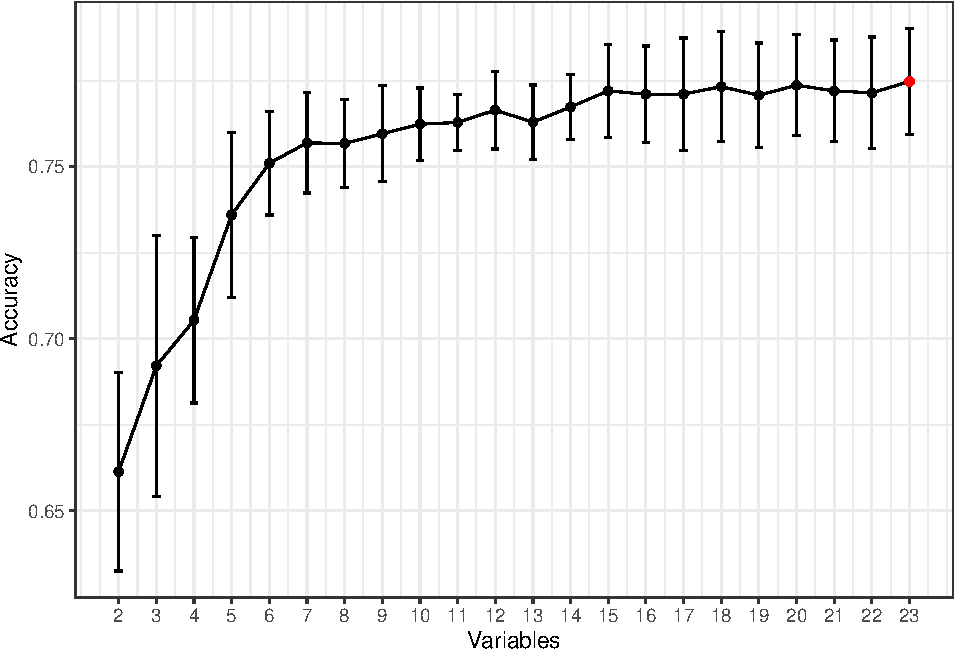
\includegraphics{seleccion_variables_experimental_analisis_files/figure-latex/rfe_evolucion_accuracy-1.pdf}

El mejor resultado se consigue con modelos que tienen las 23 variables
mencionadas anteiormente y en el grafico puede verse la evolución de
dich métrica en función de la cantidad de variables que usa con su
dispersión según todos los modelos generados con esa combinación.

Se puede observar que desde que la cantdiad de variables es 15, es un
valor muy próximo al màximo que se consigue con 23 variables. por lo que
si se opta por este tipo de dataset y se lo quisiera explicar quizas
sería mas sencillo con menos variables aunque sigue siendo una catiadd
considerable y dependerá mucho de la interacción entre ellas.

Tras ajustar cada modelo, se recalcula la influencia de cada variable.
De esta forma, para cada tamaño de modelo, se obtiene un ranking de la
importancia promedio de las variables.

\begin{table}[!h]

\caption{\label{tab:tf_rfe_influencia_variables_23}Influencia de variables en el resultado}
\centering
\begin{tabular}[t]{lrr}
\toprule
\rowcolor{black}  \multicolumn{1}{c}{\textcolor{white}{\textbf{var}}} & \multicolumn{1}{c}{\textcolor{white}{\textbf{media\_influencia}}} & \multicolumn{1}{c}{\textcolor{white}{\textbf{sd\_influencia}}}\\
\midrule
\rowcolor{gray!6}  tipo\_de\_aprobacion\_libre & 50.79648 & 2.5524875\\
Turno\_Tarde & 44.59747 & 0.8908022\\
\rowcolor{gray!6}  Turno\_Noche & 43.09091 & 1.1487629\\
tipo\_de\_aprobacion\_no\_firmo & 42.65281 & 1.5211102\\
\rowcolor{gray!6}  Aprobado & 42.15115 & 2.1368377\\
\addlinespace
tipo\_de\_aprobacion\_firmo & 40.75425 & 1.1106366\\
\rowcolor{gray!6}  Turno\_Manana & 40.69317 & 1.9193145\\
Nota\_max\_prom & 40.54109 & 1.7290803\\
\rowcolor{gray!6}  cant\_recursada\_regular\_No\_Recurso & 36.59649 & 1.7624988\\
cant\_resursada\_regular & 36.06834 & 1.6028767\\
\addlinespace
\rowcolor{gray!6}  edad\_al\_ingreso & 34.36706 & 2.0057595\\
cant\_recursada\_regular\_Recurso1vez & 33.45997 & 1.0793458\\
\rowcolor{gray!6}  noAprobado & 32.05701 & 1.4956207\\
tipo\_de\_aprobacion\_cambio\_curso & 32.04880 & 1.2241621\\
\rowcolor{gray!6}  tipo\_de\_aprobacion\_promociono & 30.37739 & 0.4212574\\
\addlinespace
Promociono & 30.31098 & 1.9463734\\
\rowcolor{gray!6}  Nota & 30.01460 & 1.9773123\\
EsTecnico\_X1 & 24.08818 & 1.1924095\\
\rowcolor{gray!6}  cant\_recursada\_regular\_Recurso2vez & 23.93968 & 1.2196074\\
Sexo\_M & 18.84818 & 2.2983891\\
\addlinespace
\rowcolor{gray!6}  cant\_recursada\_regular\_Recurso3vez & 17.05511 & 1.4083702\\
EsTecnico\_SinDato & 16.70716 & 1.3843021\\
\rowcolor{gray!6}  cant\_recursada\_regular\_Recurso4vez & 13.33266 & 1.3074133\\
\bottomrule
\end{tabular}
\end{table}

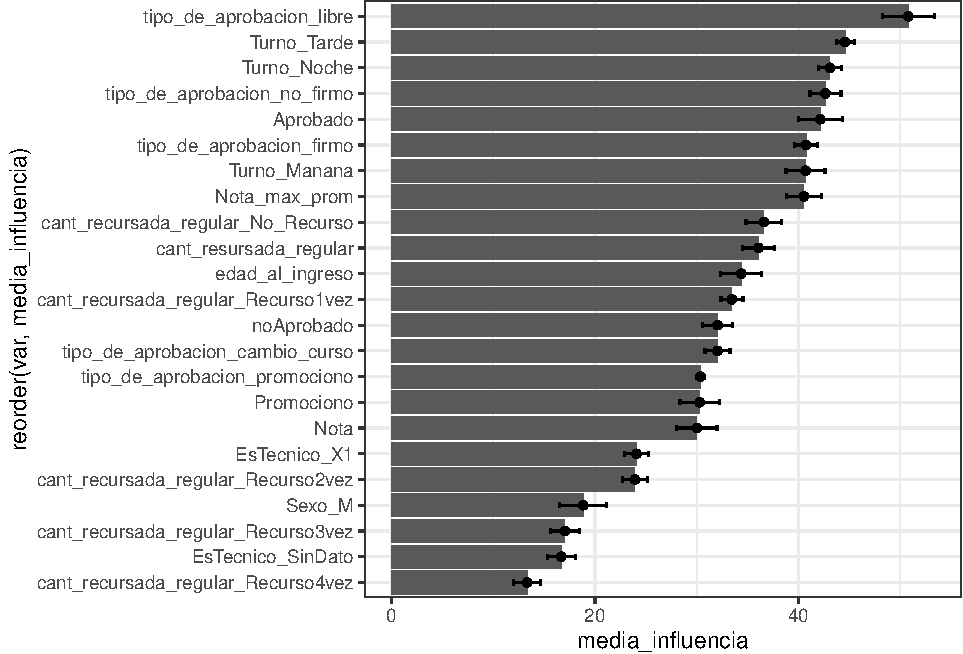
\includegraphics{seleccion_variables_experimental_analisis_files/figure-latex/influencia_de_variables_23-1.pdf}

\end{document}
